\section{Introduction}

The transition from static language models to autonomous agents marks a pivotal shift in artificial intelligence, enabling systems to handle complex, dynamic tasks through iterative reasoning and tool use~\citep{cheng2024exploring,tao2024survey,gao2025survey,fang2025comprehensive}. 
To facilitate continuous improvement without expensive parameter retraining, \textbf{procedural memory}—which internalizes ``how-to'' knowledge from past interactions—has emerged as a critical substrate for agent evolution~\citep{zhang2025survey,xu2025mem}. 
By accumulating high-quality problem-solving experiences, agents can leverage prior successes to navigate novel scenarios, theoretically reducing redundant trial-and-error and circumventing local optima~\citep{wang2025mirix,chen2025swe}.

To bridge the gap between static storage and dynamic reasoning, an ideal procedural memory system must function not merely as a database, but as an evolving cognitive substrate satisfying three core criteria:
(1) \textbf{High-Fidelity Extraction}: The system should distill generalized principles from noisy execution traces, ensuring that stored memories represent high-quality causal knowledge rather than raw observations.
(2) \textbf{Context-Adaptive Utilization}: Retrieved memories must be dynamically adapted to the nuances of the current task, maximizing their utility in novel scenarios.
(3) \textbf{Timely Evolution}: The memory pool must maintain its vitality through continuous updates, autonomously reinforcing effective strategies while purging obsolete entries to prevent degradation over time.

However, despite the promise of memory-augmented agents, current frameworks often fall short of these ideals, predominantly suffering from a \textbf{``passive accumulation''} paradigm. 
Prevailing approaches typically treat memory as a static append-only archive, storing raw, trajectory-level interactions~\citep{zheng2023synapse,hu2024hiagent} or generalized workflows~\citep{tang2025agentkb,liu-etal-2025-contextual}. 
This introduces fundamental limitations:
\textit{Abstraction Deficit}, where retaining entire trajectories introduces instance-specific noise that dilutes critical reasoning signals, preventing the agent from grasping the core logic; % Modified here
\textit{Rigid Retrieval}, where fetched experiences are applied without adaptation, leading to failures in slightly shifted contexts;
and crucially, \textit{Lack of Maintenance}, where the absence of timely update strategies causes the memory pool to degrade into a mixture of valid insights and toxic noise~\citep{xiong2025memory}.
\begin{figure*}
    \centering
    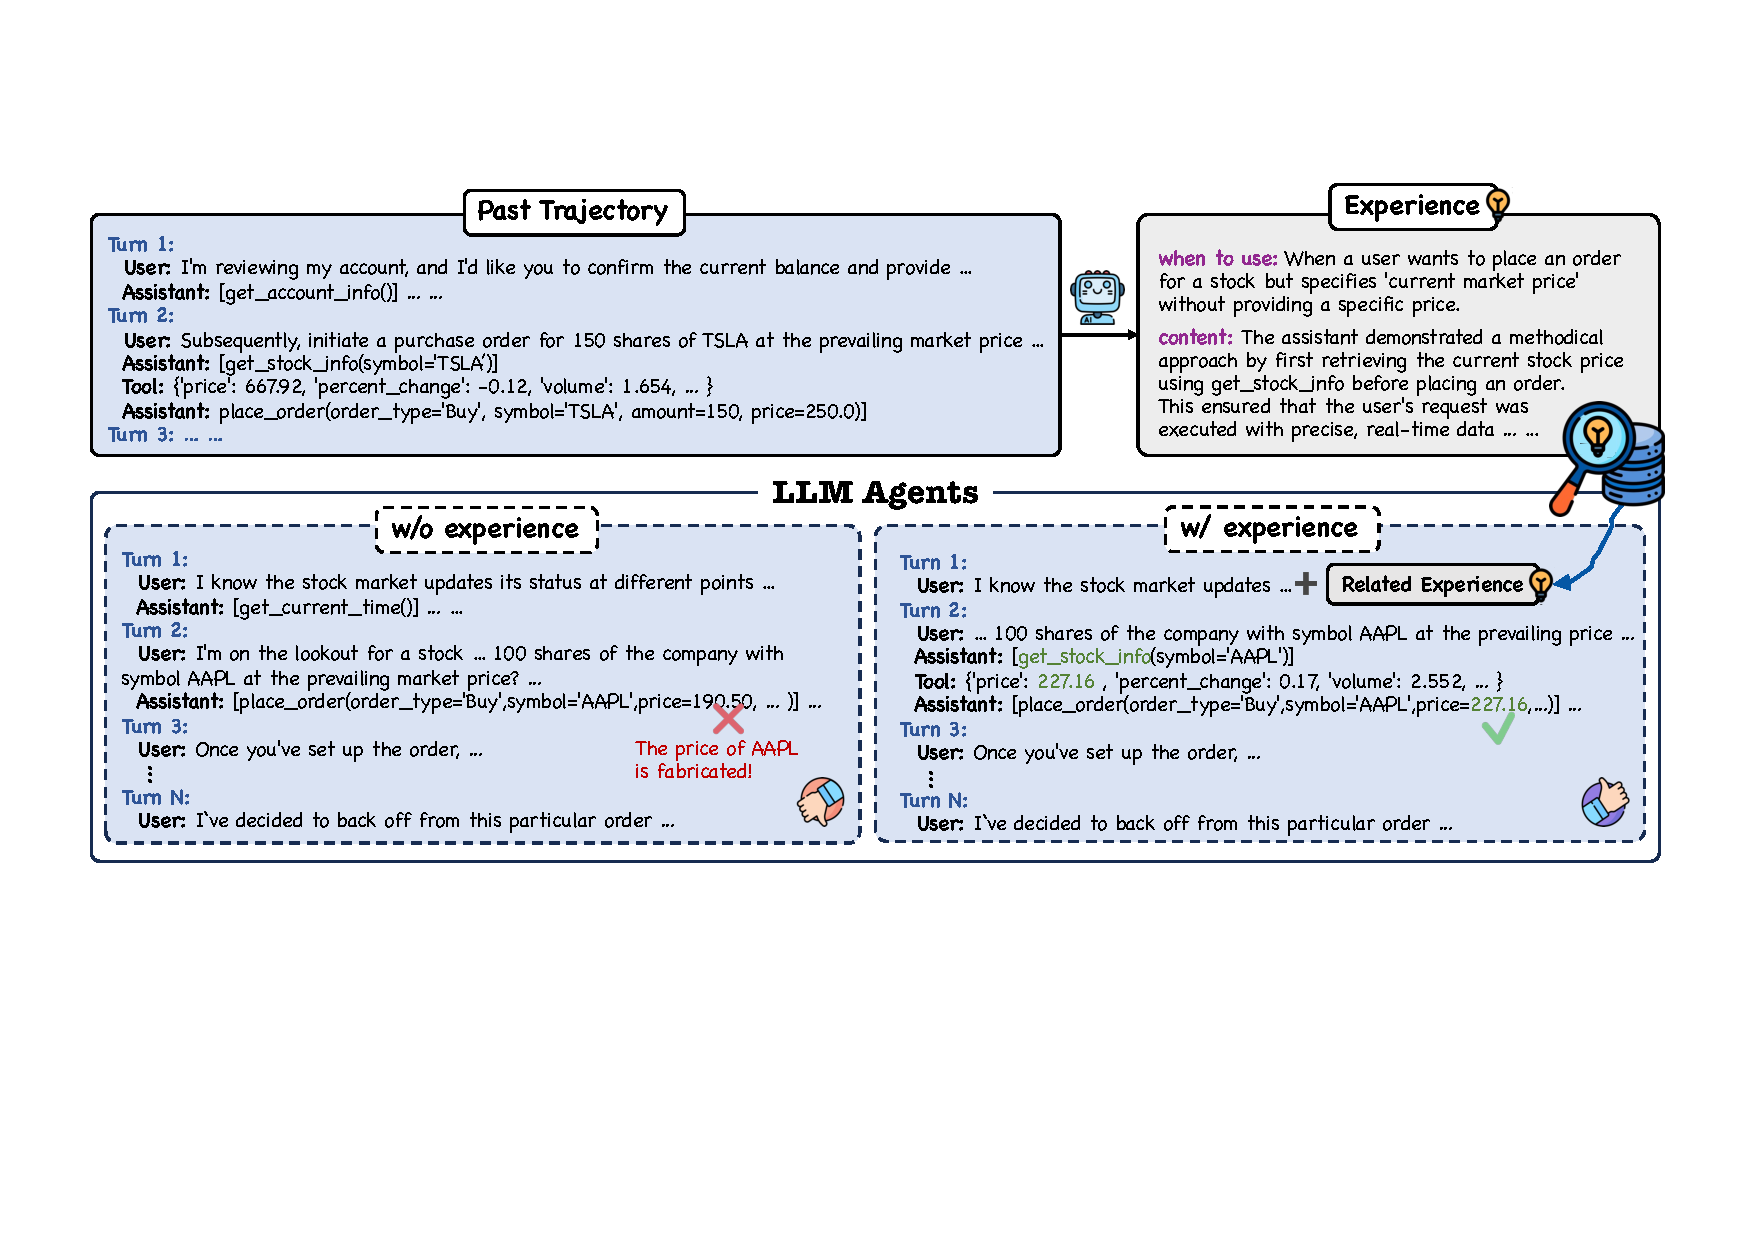
\includegraphics[width=1\linewidth]{figures/example.pdf}
    \caption{Example of how agents complete one stock trading task with and without past experience.}\label{fig:example}
\end{figure*}

To address these challenges, we propose \textbf{\ours} (\textit{Remember Me, Refine Me}), a dynamic framework that shifts the paradigm from passive storage to \textbf{feedback-driven experience evolution}. 
We systematically innovate across the memory lifecycle to meet the criteria of an ideal system.
First, for \textit{High-Fidelity Extraction}, {\ours} employs a \textbf{contrastive distillation strategy}. By analyzing the divergence between successful and failed attempts, the system isolates \textbf{pivotal decision points}—the specific strategic moves that differentiate high-quality outcomes from suboptimal ones—thereby maximizing the signal-to-noise ratio.
Second, for \textit{Context-Adaptive Utilization}, we design a comprehensive reuse pipeline. Beyond simple retrieval, this module employs \textbf{reranking and adaptive rewriting} to tailor historical insights to the specific constraints of new tasks, supplemented by a \textbf{failure-aware reflection} protocol to dynamically adjust reasoning paths when direct application proves insufficient.
Finally, for \textit{Timely Evolution}, {\ours} implements a \textbf{utility-based refinement mechanism}. Treating the memory pool as a living ecosystem, our framework tracks the utility of each experience during reuse, autonomously pruning entries that fail to contribute to task success to maintain a compact and highly effective memory state.

Our extensive experiments on BFCL-V3 and AppWorld benchmarks demonstrate that {\ours} establishes a new state-of-the-art for memory-augmented agents. 
Most notably, our results reveal that memory quality can substitute for model scale: \textbf{{\ours} enables a Qwen3-8B model to outperform a parameter-heavier Qwen3-14B baseline (without memory)}, achieving average gains of 10.65\% in Avg@4. 
These findings suggest that a self-evolving memory mechanism offers a computationally efficient pathway for lifelong agent learning.

In summary, our contributions are as follows:
\begin{itemize}[leftmargin=12pt,topsep=2pt,itemsep=2pt]
    \item We propose \textbf{\ours}, a comprehensive framework for agent evolution that integrates contrastive experience distillation, context-adaptive reuse, and utility-driven refinement. This closes the loop of procedural memory, resolving the ``passive accumulation'' dilemma by enabling agents to autonomously distill, adapt, and maintain high-quality reasoning patterns.
    
    \item We release \textbf{\texttt{reme.library}}, a fine-grained procedural memory dataset constructed from diverse agentic tasks. Containing structured success patterns and failure lessons, this library serves as a valuable resource for the community to study procedure memory and optimize memory-augmented agents.
    
    \item Extensive experiments show that {\ours} significantly enhances agent performance across diverse benchmarks. Crucially, we demonstrate a \textbf{memory-scaling effect}, where smaller models equipped with {\ours} surpass larger baselines, validating our framework as a computationally efficient pathway for lifelong agent learning.
\end{itemize}
